\documentclass{article}
\usepackage{import}
\subimport{../}{preamble}
\begin{document}

\section{Electronics Design}

By applying a voltage, \gls{V}, and measuring the current, \gls{I}, the conductance of a tunnel junction between tips can be determined using $I=\gls{G}V$. From this macroscopic value the underlying quantum tunnelling transmission can be seen and correlated with optical measurements to gain a sense of spatial separation and the extent of charge transfer across the gap. % should this be G=dI/dV

\begin{figure}[bt]
\centering
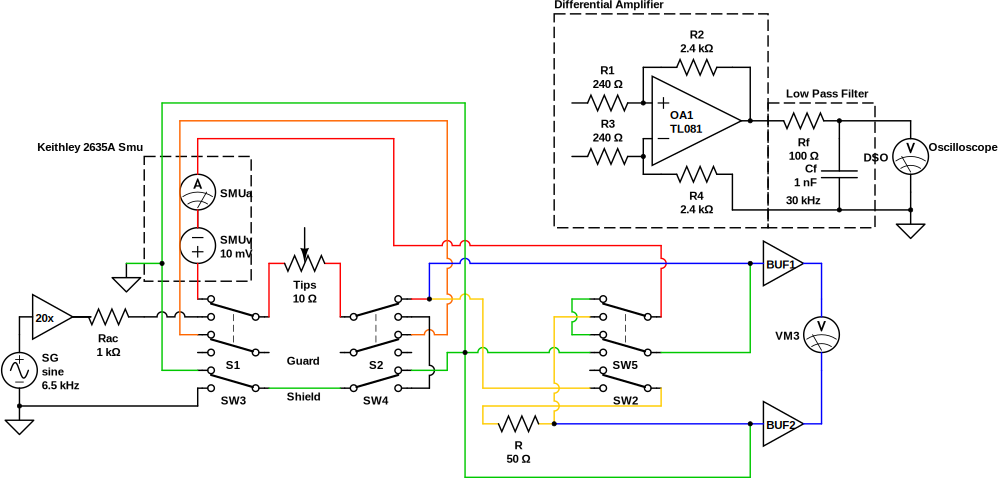
\includegraphics[width=0.9\textwidth]{figures/tip_experiment_circuit_design}
\caption[Schematic of the electrical measurement circuit.]{\textbf{Schematic of the electrical measurement circuit.} The central routing box allows switching between a.c.\ and d.c.\ circuits and low-and high-bandwidth d.c.\ measurements. The a.c.\ circuit is used to align two AFM probes together while the d.c.\ circuit is used to measure spatially dependent signals from the gap between two AFM probes.}
\label{fig:circuit_design}
\end{figure}

% Chamber electronics and routing box
The experimental chamber contains two triaxial connectors, one attached to each Cu tip clamp, to send and return electronic signals, permitting biasing and electrical measurement of the gap between \gls{afm} tips. Electronic signals are controlled and {\color{red}redirected/routed} using a control box, which attaches to the chamber triax cables. Electronics are split between an a.c.\ circuit that drives a resonant capacitive tip alignment procedure and a d.c.\ circuit for electrical measurements. The d.c.\ electronics are further split into low and high bandwidth measurement circuits. The low bandwidth ($<\SI{10}{Hz}$) circuit measures electronics continually over long time periods, typically giving spatial information linked to sample separation. The high bandwidth circuit operates on a trigger to capture single shot events on much shorter time scales. The d.c.\ circuits are typically ran simultaneously while the a.c.\ and d.c.\ circuits are manually switchable. The schematic of this system is shown in \figurename~\ref{fig:circuit_design}.

% Circuits
The a.c.\ circuit consists of a signal generator connected to a 20$\times$ voltage amplifier to drive the junction capacitance. This is used to resonantly drive an AFM cantilever into oscillation and align tips into a tip-to-tip dimer configuration. A \SI{40}{\kilo\ohm} current limiting resistor is placed after the amplifier to prevent damage to the tip junction in the event of a direct conductive contact.% actually change the resistor from 200 ohm
\footnote{The optimum resistance value is calculated using $R = V/I_{\mathrm{limit}}$ where $V=\SI{10}{V}$ typically and a safe current limit is $I_{\mathrm{limit}}=\SI{250}{\micro\ampere}$. This gives a resistance of \SI{40}{\kilo\ohm}.}
The return signal from the circuit is then terminated at ground. The separate d.c.\ circuit consists of a \gls{smu} circuit for low-bandwidth (sub-\SI{10}{Hz}) measurements with a switchable high-bandwidth measurement extension. The \gls{smu} (Keithley 2635A) is used to apply a voltage across the junction and measure the current. The switchable high-bandwidth path routes the current through a \num{e4}$\times$ gain transimpedance amplifier (Femto DLPCA-200) and then a \SI{1}{MHz} low-pass filtering stage (SRS SR560). The amplified voltage is measured on a \gls{dso} (Agilent DSOX-2012) with the shield becoming the return path of the current back to the \gls{smu} via the routing box.%
\footnote{An alternative strategy for converting a current into a voltage is to pass the current through a well-known resistor and differentially amplify the voltage drop across the resistor. This was not used since the transimpedance amplifier was readily available and of a low noise specification.}

% Circuit separability to reduce noise
The fundamental feature of combined circuity is their separability. The a.c.\ circuit is not required to be low-noise but the d.c.\ circuitry is used to measure low-level tunnelling currents. For the d.c.\ circuit to operate correctly it must be isolated from any other electronics. The a.c.\ circuit remains completely disconnected and held at ground when the d.c.\ circuit is engaged, and vice-versa.
% Other considerations to reduce noise
To achieve measurements of small, sensitive currents, reducing the noise level to a minimum is imperative. The noise floor at low bandwidths, along with the current range of the \gls{smu}, sets the minimum current which can be measured. The sub-\SI{10}{Hz} bandwidth of the \gls{smu} removes much of the noise during spatial measurements. Correct grounding of of all electronic chassises to a single point (the \gls{smu}) shields \gls{emi} and prevents ground loops from inducing current offsets. Triax cabling is used with guarded connections where possible to prevent leakage currents.

A standard operating voltage between 10--\SI{50}{mV} is used to drive high quality tunnelling currents. Using lower voltages means currents are only observable for larger tunnelling conductances, i.e.\ smaller gap widths, whilst higher voltages lead to larger overall currents and electrostatic interaction between tips, both of which should be avoided to prevent damage to the tip junction. To maintain good scan speeds the current range is restricted to \SI{10}{nA} with a \SI{\pm10}{pA} error, since more accurate ranges have longer settling times. Limiting the current range is the dominant source of current measurement error as opposed to the noise floor.

%\begin{figure}[bt]
%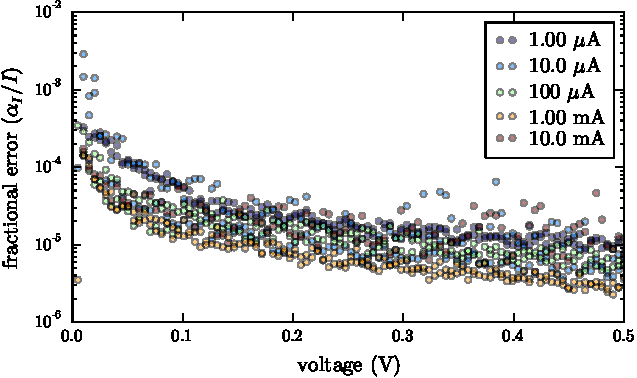
\includegraphics{figures/dc_noise}
%\caption[]{}
%\label{fig:dc_noise}
%\end{figure}

Noise on the \gls{smu} is measured by varying a series resistance in place of the tip junction and taking the standard deviation of 20 measurements across a range of voltages in \SI{10}{mV} steps. The open circuit noise measures \SI{\pm10}{pA}. Johnson noise for such a circuit is estimated to be around \SI{1}{pA}.
%The fractional errors (standard deviations normalised to the mean) measured at each voltage for each resistance (represented by the \gls{smu} current range) are shown in \figurename~\ref{fig:dc_noise}.
If current measurements are strictly limited by the current range then the percentage error of each range should be equivalent. This is not the case, with the percentage error increasing from \num{e-3}\% to \num{e-2}\% as the current decreases to the nA range, signifying the approach of the noise floor. Actual noise levels around \SI{\pm100}{pA} are found at \SI{50}{mV} with a \SI{1}{\mega\ohm} junction resistance characteristic of electron tunnelling. Given the small percentage errors, circuit noise is not a problem for tunnelling current measurements.

Noise predominantly affects high bandwidth measurements, where it limits the conductance resolution and minimum trigger level for single shot measurements. High bandwidth noise typically originates from digital circuitry, e.g.\ switch-mode power supplies and powered relays. Power supplies are therefore covered in foil to shield \gls{emi} and manual toggle switches are used instead of remote-controlled relays. Applying a \SI{1}{MHz} filter goes some way to reducing high bandwidth noise. Any more filtering smooths measurements too much.

\begin{figure}[bt]
\centering
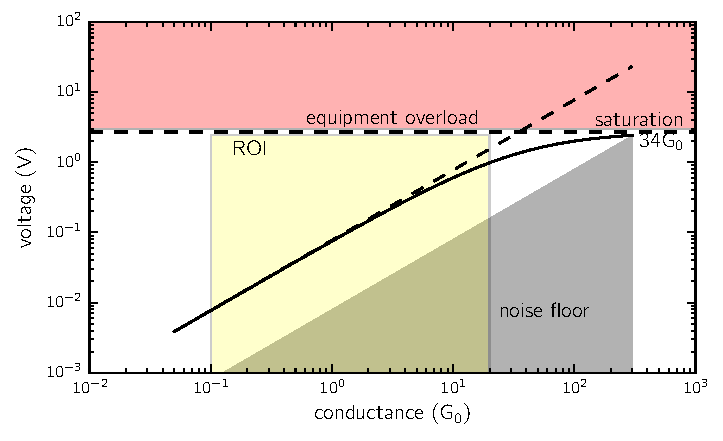
\includegraphics{figures/hb_electronics_limits}
\caption[Characterisation of electronic measurements based on junction conductance.]{\textbf{Characterisation of electronic measurements based on junction conductance.} Solid lines show the calculated SMU currents and amplified voltages for given junction conductances under a \SI{50}{mV} applied voltage with a \SI{241}{\ohm} current limiting resistor to prevent saturation (high bandwidth circuit). Dashed lines show the calculated oscilloscope voltages for the case without the current limiting resistor (low bandwidth circuit). Circles mark experimentally measured points using resistors in place of the junction in both circuits. Error bars are present but too small to visibly see.}
\label{fig:hb_electronics_limits}
\end{figure}

The maximum allowed current is set to \SI{250}{\micro\ampere} to prevent damage to contacted \gls{afm} tips. Upon surpassing this limit the \gls{smu} attenuates the voltage to reduce the current. A current limiting resistor is also included in the circuit the ensure a hardwired maximum and to prevent overloading of the \gls{dso} and transimpedance amplifier. The value of this resistor is calculated using,
\begin{equation}
R = \frac{AV}{0.95V_{\mathrm{overload}}},
\end{equation}
where $V$ is the operating voltage, $A$ is the amplifier gain and $V_{\mathrm{overload}}$ is the minimum overload voltage for the circuit at a given voltage $V$ (determined by whichever overload voltage is surpassed first, either the maximum transimpedance input current of \SI{5}{mA} pre-amplification or the maximum output voltage of \SI{5}{V}). The pre-factor of 0.95 is used to prevent the current getting close to overloading. For a \SI{50}{mV} bias and \num{e4} gain the ideal resistance is \SI{175}{\ohm} but for a \SI{10}{mV} bias with \num{e5} gain the idea resistance becomes \SI{350}{\ohm}. To accommodate a range of voltages and both gain settings, a middle resistance of \SI{241}{\ohm} is used, which provides some headroom for increasing the voltage. The calculated current and \gls{dso} voltage as a function of junction conductance for the low and high bandwidth circuits is shown in \figurename~\ref{fig:hb_electronics_limits}. Excellent agreement with experimental current and voltage measurements taken with a set of resistors demonstrates the circuit behaves exactly as predicted.

The presence of the current limiting resistor means that measured circuit conductances, $G_{\mathrm{measured}}$, contain a series resistance that needs to be taken into account. Junction conductances are calculated using,
\begin{equation}
	G_{\mathrm{junction}} = \left(G_{\mathrm{measured}}^{-1} - R\right)^{-1}.
\end{equation}
The maximum conductance value that can be measured is found by inverting the limiting resistance using $G_{\mathrm{max}} = 1/R$. For a \SI{50}{mV} bias the conductance limit is 53\G0. Conductances greater than this value are small compared to the series resistance and are therefore much harder to measure reliably. For this reason the range of interesting conductances ($G<20\G0$) is ideally kept to the linear part of the current curve by limiting the voltage and gain.

\FloatBarrier
\end{document}